% Copyright 2018  Ed Bueler

\documentclass[10pt,hyperref]{beamer}

\mode<presentation>
{
  \usetheme{Madrid}

  \usecolortheme{beaver}

  \setbeamercovered{transparent}
  
  \setbeamerfont{frametitle}{size=\large}
}

\setbeamercolor*{block title}{bg=red!10}
\setbeamercolor*{block body}{bg=red!5}

\usepackage[english]{babel}
\usepackage[latin1]{inputenc}
\usepackage{times}
\usepackage[T1]{fontenc}
% Or whatever. Note that the encoding and the font should match. If T1
% does not look nice, try deleting the line with the fontenc.

\usepackage{empheq}
\usepackage{animate}
\usepackage{xspace}
\usepackage{verbatim,fancyvrb}
\usepackage{hyperref}

% If you wish to uncover everything in a step-wise fashion, uncomment
% the following command: 
%\beamerdefaultoverlayspecification{<+->}

\newcommand{\bb}{\mathbf{b}}
\newcommand{\bc}{\mathbf{c}}
\newcommand{\br}{\mathbf{r}}
\newcommand{\bx}{\mathbf{x}}
\newcommand{\by}{\mathbf{y}}
\newcommand{\bv}{\mathbf{v}}
\newcommand{\bu}{\mathbf{u}}
\newcommand{\bw}{\mathbf{w}}

\newcommand{\grad}{\nabla}

\newcommand{\CC}{\mathbb{C}}
\newcommand{\RR}{\mathbb{R}}

\newcommand{\ddt}[1]{\ensuremath{\frac{\partial #1}{\partial t}}}
\newcommand{\ddx}[1]{\ensuremath{\frac{\partial #1}{\partial x}}}
\renewcommand{\t}[1]{\texttt{#1}}
\newcommand{\Matlab}{\textsc{Matlab}\xspace}
\newcommand{\Octave}{\textsc{Octave}\xspace}
%\newcommand{\MO}{\Matlab/\Octave}
\newcommand{\MO}{\Matlab}
\newcommand{\eps}{\epsilon}

\newcommand{\MS}{\alert{MAKE SURE}\xspace}

\newcommand{\exer}[2]{\medskip\noindent \textbf{#1.}\quad #2}

\newcommand{\mfile}[1]{
\VerbatimInput[frame=single,label=\fbox{\scriptsize \textsl{\,#1\,}},fontfamily=courier,fontsize=\scriptsize]{#1}
}

\newcommand{\mfiletiny}[1]{
\VerbatimInput[frame=single,label=\fbox{\scriptsize \textsl{\,#1\,}},fontfamily=courier,fontsize=\tiny]{#1}
}

\AtBeginSection[]
{
  \begin{frame}<beamer>
    \frametitle{Outline}
    \tableofcontents[currentsection,hideallsubsections]
  \end{frame}
}

\title{Steepest descent}

\subtitle{is not great}

\author{Ed Bueler}

\institute[MATH 661]{MATH 661 Optimization}

\date[Fall 2018]{1 October 2018}

\begin{document}
\beamertemplatenavigationsymbolsempty

\begin{frame}
  \maketitle
\end{frame}


\begin{frame}{steepest descent for unconstrained optimization}

\begin{itemize}
\item for the day I am away, here is a distraction from linear programming
\item these slides are a brief introduction to a well-known topic in unconstrained optimization, namely \dots
\item \alert{steepest descent}
    \begin{itemize}
    \item[$\circ$] a.k.a.~gradient descent
    \end{itemize}
\item the textbook\footnote{Griva, Nash \& Sofer, \emph{Linear and Nonlinear Optimization}, 2nd ed., SIAM Press 2009} puts it off till later but you should be aware of it now
    \begin{itemize}
    \item[$\circ$] please read sections 12.1 and 12.2, but ignore the Lemmas for now
    \end{itemize}
\end{itemize}
\end{frame}


\begin{frame}{why you should know about steepest descent}

\begin{itemize}
\item if you deal with optimization in the real world you will see it as a proposed algorithm for stuff
\item for easy problems it is the lazy-person's algorithm
        \begin{itemize}
        \item[$\circ$] ``easy'' roughly means:
            \begin{itemize}
            \item smooth
            \item dimension $< 10^6$ (or so)
            \item unconstrained
            \end{itemize}
        \item[$\circ$] \alert{I don't recommend steepest descent}
        \item[$\circ$] \dots but it might minimize total programmer time
        \end{itemize}
\item for hard problems it may be the only thing you can implement
        \begin{itemize}
        \item[$\circ$] e.g.~big machine learning problems, big nonlinear inverse problems, \dots
        \item[$\circ$] a version of steepest descent may be the standard in your industry
        \item[$\circ$] e.g.~\emph{stochastic gradient descent} is a nice, popular buzzword
            \begin{itemize}
            \item it's even slower than ordinary steepest descent
            \end{itemize}
        \end{itemize}
\end{itemize}
\end{frame}


\begin{frame}{the steepest descent algorithm}

\begin{itemize}
\item assume $f:\RR^n \to \RR$ has (at least) one continuous derivative
\item we want to solve the unconstrained problem:
    $$\min_{\RR^n} f(x)$$
\item the algorithm:

\medskip
\mbox{\parbox{\textwidth}{%
\begin{itemize}
\item[1.] User supplies $x_0$.
\item[2.] For $k=0,1,2,\dots$
    \begin{itemize}
    \item[(i)] If $x_k$ is optimal then stop.
    \item[(ii)] Search direction is
       $$p_k = - \grad f(x_k)$$
    \item[(iii)] Determine step length $\alpha_k>0$.  Let $x_{k+1}=x_k+\alpha_k p_k$.
    \end{itemize}
\end{itemize}%
}}

\end{itemize}
\end{frame}


\begin{frame}{steepest descent is obvious}

\begin{itemize}
\item it is an \emph{obvious} interpretation of general optimization algorithm II in \S 2.4
    \begin{itemize}
    \item[$\circ$] direction is chosen as ``go straight downhill''
        \begin{itemize}
        \item recall from calculus: the gradient points straight uphill
        \end{itemize}
    \item[$\circ$] but we don't know how to use the length of $\grad f(x_k)$
    \item[$\circ$] \dots so we \emph{must} make a choice for $\alpha_k$
    \item[$\circ$] also we need a stopping criterion
    \end{itemize}

\medskip
\item \emph{any} choice of steepest descent length, i.e.~$p_k = - c \grad f(x_k)$ and $c>0$, generates a (feasible) descent direction at $x_k$
    \begin{itemize}
    \item[$\circ$] recall: $p$ is a \emph{descent direction at} $x$ if $p^\top \grad f(x)<0$
    \end{itemize}

\medskip
\item choosing $p_k = - \grad f(x_k)$ uses the direction which solves this directional-derivative optimization problem
    $$\min_{\|q\|=1} q^\top \grad f(x_k)$$
\end{itemize}
\end{frame}


\begin{frame}[fragile]{one way to choose step length: back-tracking}

\begin{itemize}
\item we will see in section 11.5 that we can prove convergence of many unconstrained optimization algorithms as long as the step-size $\alpha_k$ is chosen to satisfy certain conditions
\item for now I just need \emph{some} reasonable way to choose $\alpha_k$
\item the standard way to satisfy these conditions is called ``back-tracking''
    \begin{itemize}
    \item[$\circ$] page 378 of the textbook
    \item[$\circ$] an implementation:

\medskip
\begin{Verbatim}[fontsize=\scriptsize]
    function alpha = bt(xk,pk,dfxk,f)
    Dk = dfxk' * pk;     % scalar directional derivative; negative
    c = 1.0e-4;          % modest sufficient decrease
    rho = 0.5;           % backtracking by halving
    alpha = 1.0;
    while f(xk + alpha * pk) > f(xk) + c * alpha * Dk
        alpha = rho * alpha;
    end
\end{Verbatim}

\medskip
    \item[$\circ$] we will return to this topic
    \end{itemize}
\end{itemize}
\end{frame}


\begin{frame}[fragile]{steepest-descent-back-tracking code}

\begin{itemize}
\item here is a basic implementation of \emph{steepest-descent-with-back-tracking}
    \begin{itemize}
    \item[$=$] SDBT
    \end{itemize}
\item it assumes that the user supplies $x_0$ and a function $f$ that returns both the values $f(x)$ and the gradient $\grad f(x)$:

\medskip
\begin{Verbatim}[fontsize=\small]
xk = x0;
for k = 1:maxiters
    [fxk, dfxk] = f(xk);
    if norm(dfxk) < tol
        break
    end
    pk = - dfxk;                % steepest descent
    alpha = bt(xk,pk,dfxk,f);   % back-tracking
    xk = xk + alpha * pk;
end
\end{Verbatim}

\medskip
\item you can set \texttt{maxiters} to $10^4$ or so to avoid long waits for failure
\end{itemize}
\end{frame}


\begin{frame}{steepest-descent-back-tracking: example I}

\begin{itemize}
\item suppose $f(x) = 5 x_1^2 + \frac{1}{2} x_2^2$ for $x\in\RR^2$, an easy quadratic objective function with global minimum at $x^*=(0,0)^\top$
\item result from SDBT:

\begin{center}
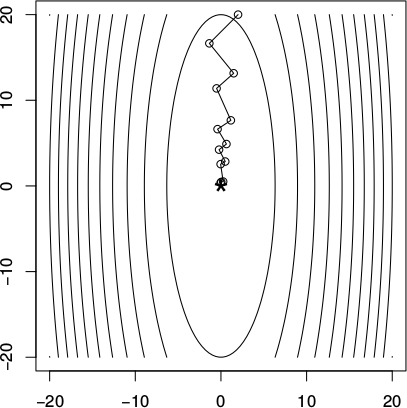
\includegraphics[width=0.4\textwidth]{egg-sd-backtracking}
\end{center}

\medskip
\item is this result o.k.?
\end{itemize}
\end{frame}


\begin{frame}{steepest-descent-back-tracking: example II}

\begin{itemize}
\item a famously-harder problem in $\RR^2$ is to minimize the \emph{Rosenbrock function}:
    $$f(x) = 100 (x_2 - x_1^2)^2 + (1 - x_1)^2$$
    \begin{itemize}
    \vspace{-4mm}
    \item[$\circ$] is a \emph{quartic} polynomial in 2 variables
    \item[$\circ$] has a single global minimum at $x^*=(1,1)^\top$
    \item[$\circ$] has steep ``banana'' shaped contours (bottom left)
    \end{itemize}

\smallskip
\item at right: SDBT from $x_0=(0,0)^\top$
    \begin{itemize}
    \item[$\circ$] struggles
    \end{itemize}
\end{itemize}

\vspace{-8mm}

\hspace{0.3in}
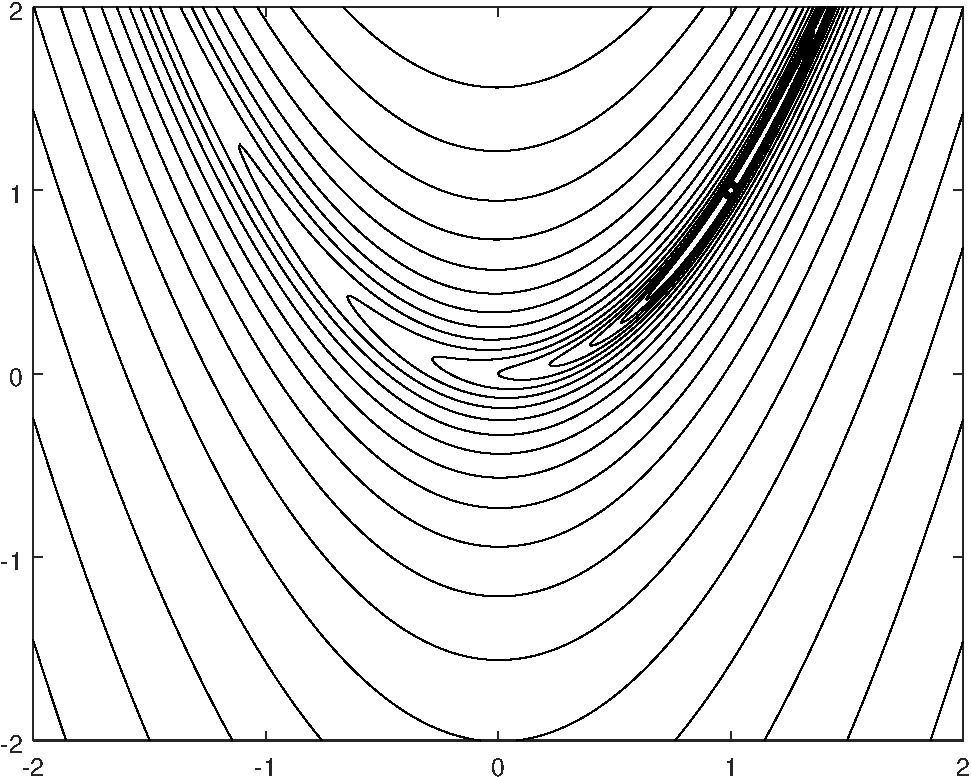
\includegraphics[width=0.35\textwidth,keepaspectratio=true]{rosencontour}
\hspace{0.3in}
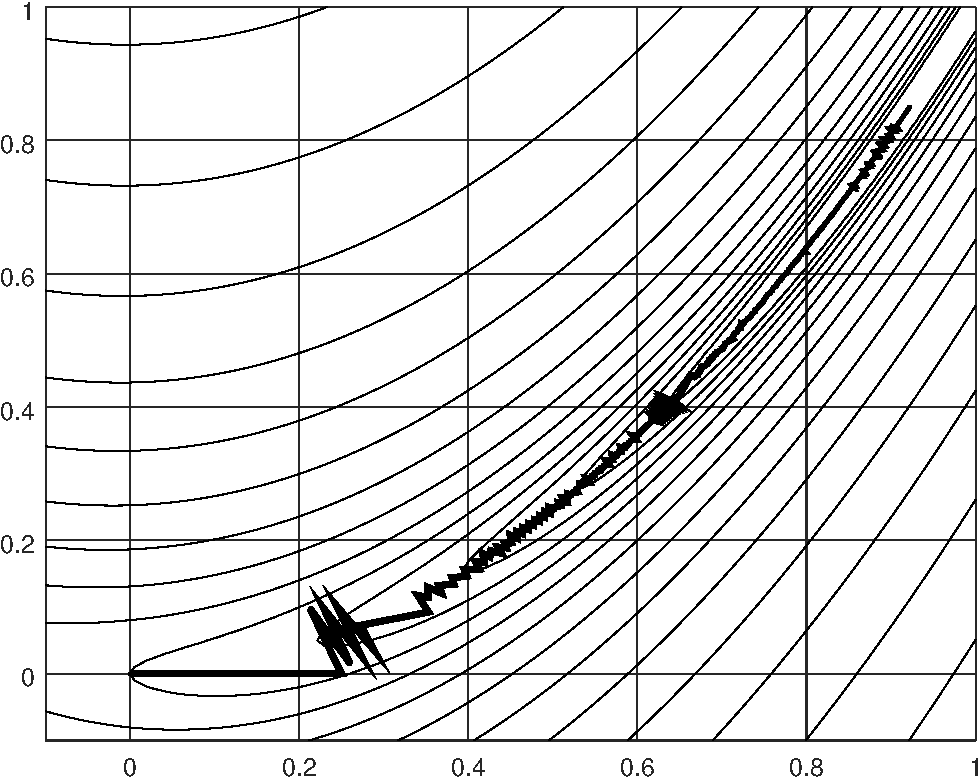
\includegraphics[width=0.46\textwidth,keepaspectratio=true]{sdrosenslow}
\end{frame}


\begin{frame}{quadratic functions}

\begin{itemize}
\item now we consider steepest descent for quadratic functions in $\RR^n$
\item such functions can always be written
    $$f(x) = \frac{1}{2} x^\top Q\, x - c^\top x + d$$
    \begin{itemize}
    \vspace{-3mm}
    \item[$\circ$] $Q$ is a symmetric square matrix, $c$ is a column vector, $d\in \RR$
    \item[$\circ$] exercise \textbf{P9} on A5: check that
        $$\grad f(x) = Q\, x - c$$
    \item[$\circ$] \emph{assume} $Q$ is positive definite
            \begin{itemize}
            \item then $f$ is strictly convex
            \item and there is unique global (and local) minimizer where $\grad f=0$: \hfill $x^* = Q^{-1} c$
            \end{itemize}
    \item[$\circ$] the additive constant $d$ can be ignored in optimization problems because it neither affects $\grad f(x)$ nor the location of $x^*$
    \item[$\circ$] example 1: $c=0$; $Q$ is a diagonal $2\times 2$ matrix with $5$,$1/2$ on diagonal
    \end{itemize}
\end{itemize}
\end{frame}


\begin{frame}{line search for quadratic functions}

\begin{itemize}
\item given any descent direction $p_k$ at $x_k$, the \emph{optimal} step size is
    $$\alpha_k = \frac{-p_k^\top \grad f(x_k)}{p_k^\top Q p_k} = \frac{p_k^\top (c - Q x_k)}{p_k^\top Q p_k}$$
    \begin{itemize}
    \item[$\circ$] showing this is in exercise \textbf{P9} on A5
    \end{itemize}
\item this $\alpha_k$ minimizes $g(\alpha) = f(x_k + \alpha p_k)$ over $\alpha>0$
\item thus back-tracking is \emph{not} needed for quadratic functions

\bigskip
\item \alert{but} steepest descent is still slow
    \begin{itemize}
    \item[$\circ$] exercise \textbf{P10} on A5 asks you to reproduce Example 12.1 in section 12.2 of the textbook
    \item[$\circ$] steepest descent with optimal step size uses a totally-unnecessary 216 steps to get modest accuracy
    \item[$\circ$] since we have the optimal step size $\alpha_k$, the problem in steepest descent \alert{must be that the steepest descent direction is wrong}
    \end{itemize}

\end{itemize}
\end{frame}


\begin{frame}{steepest descent is the wrong direction}

\begin{itemize}
\item for quadratic objective functions $f(x)=\frac{1}{2} x^\top Q x - c^\top x$, where the gradient is a linear function, the \alert{Newton iteration converges to $x^*=Q^{-1}c$ in one step}
\item Newton uses this direction:
    $$p_k = - \left(\grad f(x_k)^\top\right)^{-1} \grad f(x_k)$$
\item steepest descent uses:
    $$p_k = - \grad f(x_k) = - (I)^{-1} \grad f(x_k)$$
\item unconstrained optimization usually benefits a lot from using the information in the Hessian to turn away from the steepest descent direction $-\grad f(x_k)$
    \begin{itemize}
    \item[$\circ$] that's why we will care about the rest of Chapters 11, 12, and 13
    \item[$\circ$] especially ``quasi-Newton'' methods
    \end{itemize}
\end{itemize}
\end{frame}


\begin{frame}{summary slide}

\begin{itemize}
\item steepest descent simply uses search direction $p_k = -\grad f(x_k)$
\item determining the step size $\alpha_k$ is nontrivial
    \begin{itemize}
    \item[$\circ$] line search (section 11.5) or trust region (11.6) is needed
    \item[$\circ$] for general functions, back-tracking is recommended
    \item[$\circ$] for quadratic functions we can use the optimal step size
    \end{itemize}
\item even with good line search, steepest descent sucks
    \begin{itemize}
    \item[$\circ$] steepest descent is slow when contour lines (level sets) are highly curved
    \item[$\circ$] going down the gradient is generally \alert{the wrong direction}
    \end{itemize}
\item for quadratic functions Newton is clearly better: one step convergence
\item hard functions like Rosenbrock are hard even for Newton
\end{itemize}
\end{frame}


\end{document}

